
\section{Bayesian Model}

Now we describe the setting formally. A series of competitive \textbf{rounds}, indexed by $t=1,2,3,\ldots$, take place sequentially in time. The participants of a round $t$ are a subset of all the \textbf{players}, which are indexed by $i$. At time $t$, player $i$ has latent \textbf{skill} $s_{i,t}$, which we seek to estimate from a history of observable \textbf{evidence} $e_1,\ldots,e_t$ produced by the rounds $1,\ldots,t$.

In Bayesian fashion, we start with a prior belief distribution on $s_{i,t}$ immediately preceding round $t$, taking into account all of the rounds $1,2,\ldots,t-1$. Our main task is to combine the prior belief with the evidence $e_t$ to obtain a posterior belief. This will serve as the basis for a post-round \textbf{rating}, defined to be the \textbf{maximum a posteriori} (MAP) estimate of $s_{i,t}$. That is,

\begin{align*}
r_{i,t} &= \arg\max_{s_{i,t}} f(s_{i,t} \mid e_1,\ldots,e_t) \\
&= \arg\max_{s_{i,t}} f(s_{i,t} \mid e_1,\ldots,e_{t-1}) \Pr(e_t \mid s_{i,t})
\end{align*}

where $f(s_{i,t} \mid e_1,\ldots,e_t)$ is the probability density function (p.d.f.) corresponding to our posterior belief on player $i$'s latent skill given the history of evidence. Here we used Bayes' rule to write the posterior p.d.f. as proportional to the product of the prior p.d.f. and the evidence probability.

Let's simplify the notation. Since the pre-round evidence $e_1,\ldots,e_{t-1}$ is common to both the prior and posterior beliefs, we treat them as understood and explicitly write only the new evidence $e_t$. This leaves $t$ as the only round subscript, so we omit that as well. With these changes, the post-round rating can be re-written more simply as

\[r_i = \arg\max_{s_i} f(s_i \mid e) = \arg\max_{s_i} f(s_i) \Pr(e \mid s_i)\]

We assume the evidence $e$ is produced from each round in the following generative fashion: each participant randomly draws their performance $p_i$ in the round independently from a logistic distribution centered at $s_i$, with a variance $\gamma_i^2$ that may depend on characteristics of the round $t$ (whose subscript we continue to omit) and player $i$.

While the variables $s_i$ and $p_i$ are hidden, we assume that player $i$ outranks player $j$ (written $i \succ j$) in the round if, and only if, $p_i > p_j$, and that we observe the complete relative rankings. In other words, the observable evidence $e$ consists of a total order on the set of participants.

Due to this important modeling assumption, the method is best-suited for competitions in which the most pertinent information is round rankings. Note that, in the programming contest setting, this means we discard specific information about player scores, which are difficult to model and depend heavily on the specifics of the problem set. This method would be ill-suited to model, for instance, track races, where a runner's absolute time is more informative than relative rankings. On the other hand, it may be very well-suited to obstacle-course races, if each round consists of novel obstacles that make the absolute times hard to interpret.

Strictly speaking, ties have probability zero of occurring in our model. Assuming that ties are relatively infrequent in programming contests, they can be handled with a special modification that we'll describe later, essentially treating them as half a win and half a loss.

\begin{center} 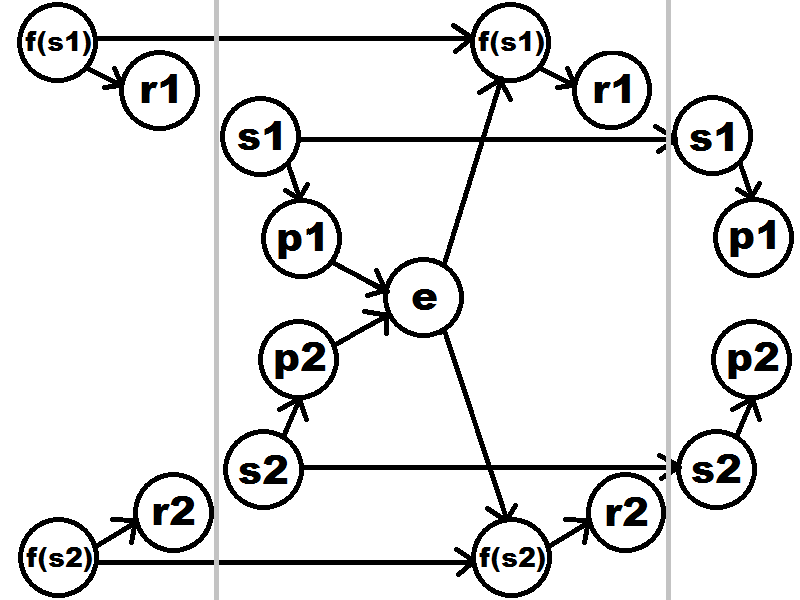
\includegraphics[scale=0.35]{../images/HMMlabeled.png} \end{center}

In order to absorb $e$ into our posterior, a few approximations are in order. First, we assume the number of participants is so large that we are able to compute the performances exactly. Mathematically, this means $\Pr(e \mid p_i)$ is proportional to a delta ``function" concentrated at the correct value of $p_i$. Hence, using Bayes' rule again,

\begin{align*}
f(s_i\mid e)
&\propto f(s_i)\Pr(e\mid s_i)
\\&= f(s_i)\int \Pr(e\mid p_i)f(p_i\mid s_i)\,dp_i
\\&\propto f(s_i)f(p_i\mid s_i)
\end{align*}

where the constants of proportionality depend on $e$ but not on $s_i$.

This suggests a natural two-phase update algorithm for each player $i$. In phase one, we estimate the MAP of $p_i$ given $e$. This estimate has very low error in the limit of very many participants, so we can take the MAP of $p_i$ to be its true value. In phase two, we update the posterior according to the above expression, and compute the new rating $r_i$ as the MAP of $s_i$ given $e$.

Note that, since the $p_i$ are assumed to be computed exactly, there is never a reason to retroactively update past estimates of performance. It follows that a round's non-participating players have posterior skill distribution identical to their prior; in particular, their ratings do not change.